\documentclass{article}

\usepackage{arxiv}
\usepackage[utf8]{inputenc}
\usepackage[T1]{fontenc}
\usepackage{url}
\usepackage{booktabs}
\usepackage{amsfonts}
\usepackage{nicefrac}
\usepackage{microtype}
\usepackage{graphicx}
\usepackage[font=small,labelfont=bf]{caption}
\usepackage{cite}
\usepackage{pdflscape}
\usepackage{listings}
\usepackage{outlines}
\usepackage{tikz}
\usepackage{epigraph}
\usepackage{natbib} 
\usepackage{url}
\usepackage{algorithm,algpseudocode}

\newcommand*\circled[1]{\tikz[baseline=(char.base)]{
		\node[shape=circle,draw,inner sep=1pt] (char) {#1};}}

\title{Lineage of tiered data in Apache Kafka}

\begin{document}
\maketitle \thispagestyle{fancy2}
\begin{abstract}
	The objective of this document is to elaborate on the design of "tiered storage" to ensure the lineage of logs in Apache Kafka is preserved  when segments are moved to and accessed from external storage tiers.
\end{abstract}

\tableofcontents

\newpage
\section{Motivation}
\epigraph{\textit{"At its heart a Kafka partition is a replicated log"}}{Apache Kafka online documentation \cite{RD1}}

As stated in the reference documentation and echoed in \cite{KDG}, replication in Apache Kafka is one of its most fundamental characteristic. The replication protocol which Kafka implements and the guarantees it provides are well documented, and explains how and why a consistent lineage for a topic-partition is preserved across its replicas irrespective of the nature and frequency of fail-overs this topic-partition experiences \cite{KIP101}\cite{KIP279}.

Over time, Kafka gracefully evolved and built on top of existing replication protocol to strengthen replication semantic. The introduction of data tiering in Apache Kafka cannot weaken it. This requires the data lineage to be kept consistent when information is read from tiered segments in addition to local segments. The specifications which apply to local replicas are still honored when tiered segments contribute to a replica's lineage.

This document assumes some level of familiarity with the replication protocol implemented in Kafka and how replica lineage is maintained across replicas. At a very high level, this protocol is based on \textit{log truncation}, which relies on replica history, materialized by a list of generation to start offset vectors, which evolves with cluster events and leadership migration. At a given point in time, the lineage of the log of a topic-partition is that of the leader replica of that topic-partition. It is possible for the end offset of the log to decrease when leadership of a topic-partition is migrated. Truncation prevents divergences between replicas.

\section{Introducing example}

The following discussion is based on an example which consists in a topic-partition with three replicas and multiple leadership migrations. The lineage tree of the topic-partition is provided in diagrams along with the leadership assignments throughout the sequence of generations for this topic-partition.

\subsection{Notations and simplifications}

\paragraph{Serialized offsets}
In this example, offsets are selected from the available replicas at points of interest. An offset is written "$\theta$" and informally indexed such that $\theta_{i+1}$ is written on a replica "after" $\theta_i$ for any given index $i$. The use of leader epochs makes this serialization possible and ensure the word \textit{after} is meaningful in this context. Note that $(\theta_i)_{i \in \mathbb{N}}$ is not necessarily monotonic. 

\paragraph{Generations}
A leader epoch is written $g$ and is indexed such that $g_{i+1}$ is "younger" than $g_i$. Note that, for simplicity, the exact sequence of incremental leader epochs is not reproduced. For instance, when replica 2 and 3 go offline in figure \ref{fig:lineage-tree-1}, the leader epoch of the topic-partition is expected to be incremented at least twice, but we will simply refer to the new leader epoch as $g_2$ even if it differs from $g_1$ by more than one logical increment.

\subsection{Lineage Tree}

\label{lineage_tree}
Figure \ref{fig:lineage-tree-1} provides the lineage tree of the log, where each replica exhibits a specific history.
The timeline of events which led to this tree are as follows:

\begin{outline}[enumerate]
\1 The root of the tree corresponds to the subsegment in the range $[\theta_1, \theta_2]$, which is assumed to be common to all three replicas.
\1 At generation $g_2$, replicas 2 and 3 become offline and replica 1 ingest records from $\theta_{2} + 1$ to beyond $\theta_3$. The segment with base offset $\theta_1$ and end offset $\theta_3$ is offloaded by replica 1\footnote{Here, the word \textit{replica} informally refers to the hosting \textit{broker}.}. The information required to know how that segment participated to the lineage of the replica needs to be preserved and leader epochs $g_1$ and $g_2$ along with start and end offsets are kept as part of the tiered segment metadata.
\1 Replica 1 becomes offline and replica 2 and 3 now contribute to the ISR set. Replica 3 is the leader. The segment with the offset range $[\theta_1, \theta_4]$ is offloaded and its generational metadata is recorded.
\1 Replica 2 falls behind and is moved out of ISR. Replica 3 continues to ingest and offload the segment ranging from offsets $[\theta_4 + 1, \theta_5]$ at generation $g_4$. This is possible because the ISR is reduced to its leader and the leader high watermark can freely moves forward.
\1 Leadership is transferred to replica 2 and replica 3 is put offline. The ISR set is now $\{2\}$. Data continues to be ingested.
\1 Replica 3 is back online. Generation is incremented to $g_6$ when it joins the cluster. Truncation is performed on the replica, which physically deletes the segment $[\theta_{5}+1, \theta_{5}+2]$. The segment the replica offloaded at generation $g_4$ is only in the external storage at truncation time. This segment is now "\textit{orphan}", because no matter the following life events affecting the cluster, there is no going back and that part of the lineage is forever discarded. Another way to see it is that the edge from the prefix $[\theta_2+1,\theta_4]$ to $[\theta_4+1,\theta_6]$ in the lineage tree can be removed.
\1 The segment $[\theta_2+1,\theta_6]$ is rolled over and eventually become eligible for tiering. It is offloaded by replica 2 and its generational metadata is recorded.
\end{outline}

The content of the tiered storage after these events is represented in figure \ref{fig:tiered-storage}, with the representation of the generational metadata associated to the tiered segments as a graph $\mathcal{G}=(\theta,g)$ which provides the ranges of offsets of the tiered segments along with the leader epochs at ingestion time.

\begin{figure}[H]
	\centering
	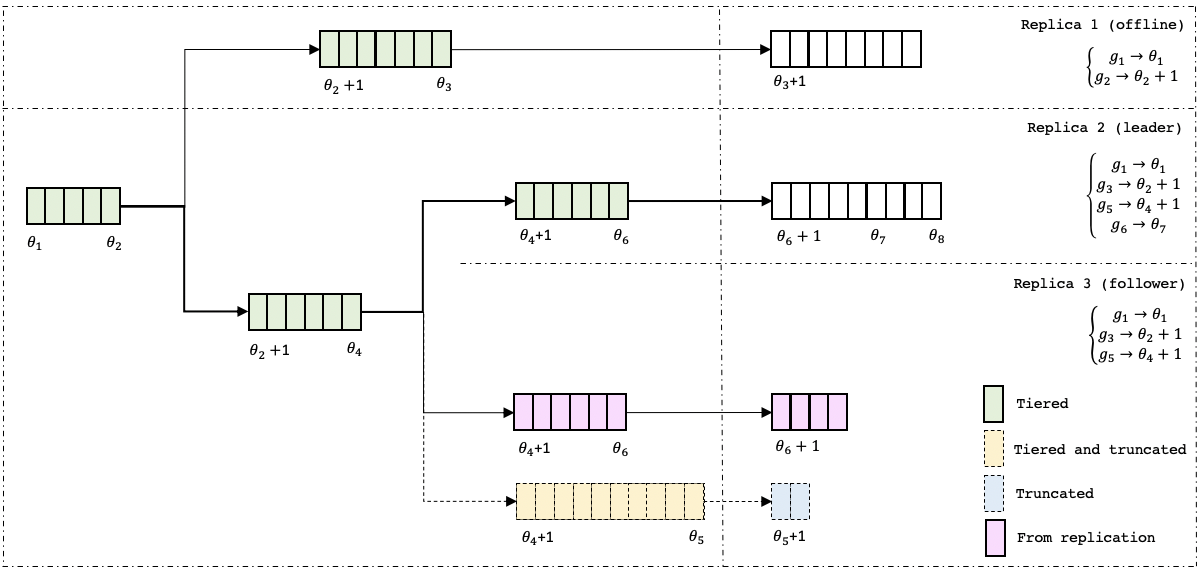
\includegraphics[scale=0.45]{lineage-tree-1.png}
	\captionof{figure}{Lineage tree of the topic-partition while replica 1 is offline. The generation-to-start-offset vectors, which build the leader epoch cache, are represented on the right.}
	\label{fig:lineage-tree-1}
\end{figure}

\begin{figure}[H]
	\centering
	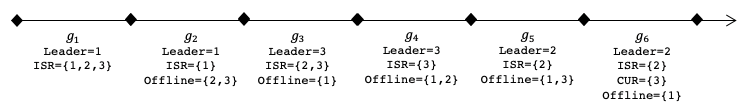
\includegraphics[scale=0.6]{seq-generations.png}
	\captionof{figure}{Lineage tree of the topic-partition while replica 1 is offline.}
	\label{fig:seq-generations}
\end{figure}

\begin{figure}[H]
	\centering
	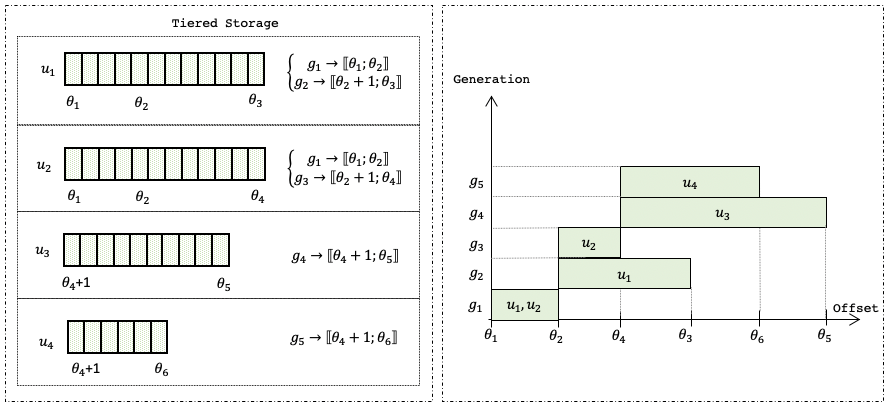
\includegraphics[scale=0.54]{tiered-storage.png}
	\captionof{figure}{On the left: tiered segments. On the right: quadrant $(\theta, g)$ associated to these segments.}
	\label{fig:tiered-storage}
\end{figure}

\newpage
\section{Lineage reconcilation with tiered segments}

\subsection{Reconcilation between local and tiered segments on \texttt{become-leader}}

\subsubsection{Tiered Aggregate}

A replica which becomes the leader of a topic-partition, and detects some segments for that topic-partition are tiered, needs to identify which parts of its lineage are present in the tiered storage. 

As such, the replica which becomes the leader of a topic-partition needs to find the latest epoch which is common to tiered segments and the local epoch cache, following an approach almost identical to the resolution of the truncation offset \cite{KIP279}. It then resolves an offset depending on the relative position of the latest offset of the tiered segments and the local end offset at generation $g$.

The similarity observed between the reconciliation of lineage in the cases of usual local replica on one hand, and tiered segments on the other hand, is not a coincidence. There is a connection in the nature of a replica and the set of tiered segments from a log of a topic-partition. While the latter is not a replica \textit{per se}, their roles in the determination of what \textit{is} the log and what its building blocks are give them a functional and operational resemblance and responsibility. This makes tiered segments much more than simple archives of earlier parts of the log.

The set of segments from a topic-partition which are offloaded to a tiered storage will be referred to as the \textbf{tiered aggregate} of the topic-partition - the result of aggregation of segments from local replicas which contributed to potentially different branches of the log lineage tree.

\paragraph{Notations}
In the following section of this document, the following notations are used to soften ambiguities. These defined are defined at the time of the resolution $g_c$ (the current leader epoch). Note that $g_c > g$.

\begin{itemize}
	\item $\theta_{t,S}(g, g_c)$ is the first offset for the generation $g$ in the tiered aggregate\footnote{Data is assumed to be physically present at that offset.}.
	\item $\theta_{t,E}(g, g_c)$ is the last offset for the generation $g$ in the tiered aggregate.
	\item $\theta_{l,S}(g, g_c)$ is the local start offset for the leader epoch $g$ (inclusive) on the leader replica.
	\item $\theta_{l,E}(g, g_c)$ is the local end offset for the leader epoch $g$ (inclusive) on the leader replica\footnote{That offset could change in case of truncation at $g' > g_c$.}.
	\item $\hat{\theta}_{l,S}(g, g_c)$ is the first offset physically present on the local storage for the generation $g$\footnote{This assumes $\theta_{l,S}(g, g_c)$ can be tracked independently from $\hat{\theta}_{l,S}(g, g_c)$. More on this later.}.
\end{itemize} 

These notations assume the underlying variables are unambiguous. For instance, $\theta_{t,E}(g, g_c)$ assumes a unique well-defined such offset throughout resolution at generation $g_c$. This may not be the case, depending on the guarantees provided by the tiering sub-system, and especially how it fences stale leaders.

\paragraph{Combinations}
A selected number of combinations of these offsets addressed during the reconciliation between the leader replica and the tiered aggregate are enumerated below and illustated on figure \ref{fig:become-leader}\footnote{
\includegraphics[scale=0.3]{tiered.png} tiered; 
\includegraphics[scale=0.3]{local.png} local.}. Not all structural configurations are considered; however, interval trichotomy (\cite{CLR} p.349) was applied to guarantee the exhaustive coverage of strutural cases involving the presence of local data (\circled{B}, \circled{C}, \circled{D}, \circled{E}, \circled{F} and \circled{G}). Not that $\theta_{t,S}(g, g_c) = \theta_{l,S}(g, g_c)$ in non-pathological cases.

\begin{figure}
	\centering
	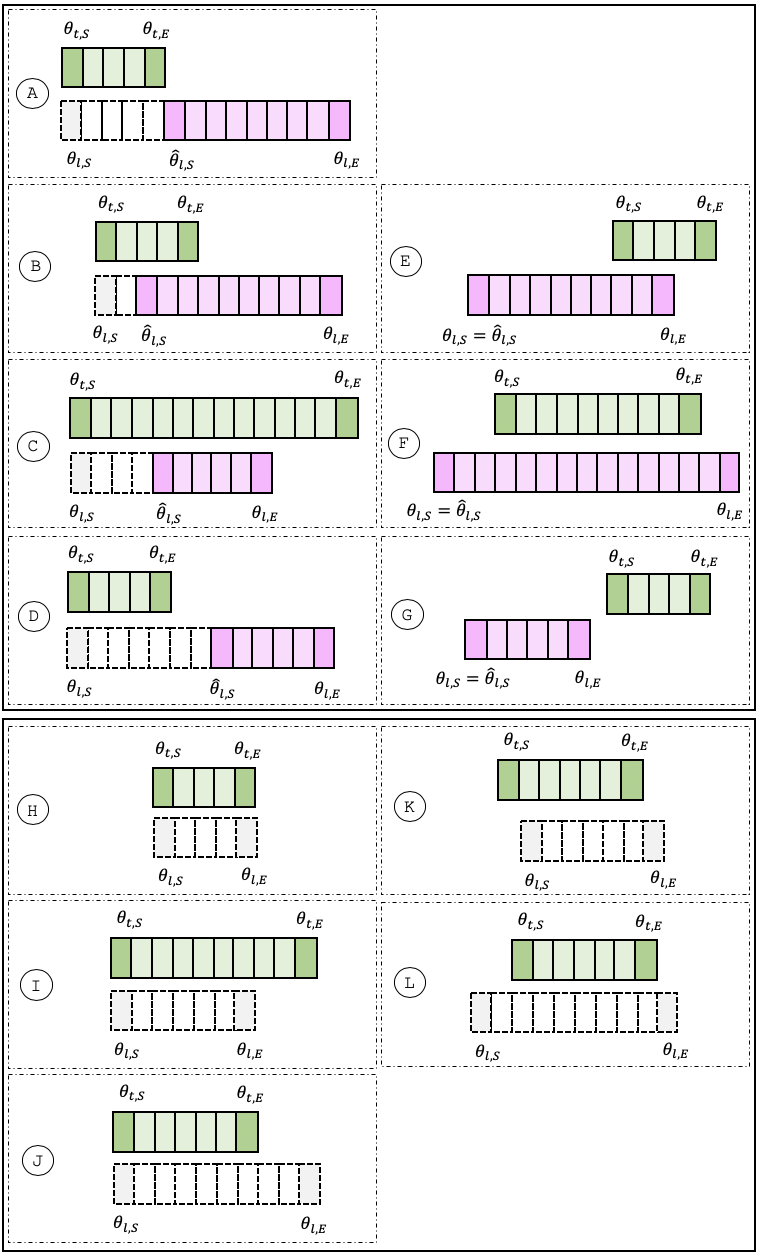
\includegraphics[scale=0.50]{become-leader.png}
	\captionof{figure}{Possible configurations between a local replica and the tiered aggregate at resolution time. Segments are not represented, only sections of the log at the generation considered. Continuity of the tiered aggregate at that generation is assumed. Generations are not written with offsets to make the notations less cluttered.}
	\label{fig:become-leader}
\end{figure}

\begin{outline}[enumerate]
	\1 \textbf{Case \circled{A}}: ${\theta}_{t,E}(g, g_c) = \hat{\theta}_{l,S}(g, g_c) - 1$. This can be a usual case encountered when leadership of the topic-partition is migrated to a previously in-sync replica subject to the same local eviction sequence as the previous leader.
	\1 \textbf{Case \circled{B}}:  $\theta_{t, S}(g, g_c) \leq \hat{\theta}_{l,S}(g, g_c) < \theta_{t,E}(g, g_c) \leq \theta_{l,E}(g, g_c)$. This can happen for instance if a tiered segment was not deleted on the new leader replica, or if the base offsets of the segments of the replica were not perfectly aligned with those of the previous leader, resulting in shifted roll-overs and deletion of local segments.
	\1 \textbf{Cases \circled{C}, \circled{I}}: $\theta_{t,S}(g, g_c) \leq \hat{\theta}_{l,S}(g, g_c) \leq \theta_{l,E}(g, g_c) < \theta_{t,E}(g, g_c)$. This can happen if the new leader replica was out of ISR before election.
	\1 \textbf{Case \circled{D}}:  $\theta_{t,E}(g, g_c) < \hat{\theta}_{l,S}(g, g_c)$. A gap separates the local start offset from the latest offset at generation $g$. This could be the result of a misconfiguration which led to the premature eviction of local segments on the new leader replica.
	\1 \textbf{Cases \circled{E}, \circled{F}, \circled{G}, \circled{L}}: $\hat{\theta}_{l,S}(g, g_c) < \theta_{t, S}(g, g_c)$. Pathological cases where the leader replica contains offsets preceding the earliest offset on the tiered storage at generation $g$. Segment tiering will ensure segments are sequentially delivered to the tiered storage, such that a segment is tiered only if the preceding segment has been successfully offloaded. However, these cases can still happen, for instance if segments were deleted from the tiered storage but kept locally on the leader replica.	
	\1 \textbf{Case \circled{H}}: Scenario where start and end offsets are perfectly aligned and no data remains on the leader replica for $g$.
	\1 \textbf{Case \circled{J}}: $\theta_{t,E}(g, g_c) < \theta_{l,E}(g, g_c)$ and data is locally absent. This case is pathological. Assuming tiering has always been enabled for the topic-partition, the tiering sub-system should ensure that the section $[1 + \theta_{t,E}(g, g_c), \theta_{l,E}(g, g_c)]$ of the log is not locally deleted if not detected as successfully tiered.
	\1 \textbf{Case \circled{K}}: A pathological case which would have required the leader replica and other replica of the topic-partition disagreed on the start offset of the generation. In order to generate this use case, one would have to enable tiering at some point in the lineage of the log and have experienced deletion of segment on a follower replica before the leader.
	\1 \textbf{Case \circled{M}}: No common epoch can be found between tiered segments and the local epochs. No segment from the log of the topic-partition has ever been offloaded to the tiered storage.
\end{outline}

\paragraph{Remark 1}
In order to ensure the resolution of the latest generation shared by the leader replica and the tiered aggregate is possible in the absence of local segment for that generation, the full history of the generations of the local replica needs to be available. Currently, when segments are locally deleted, the earliest offset of the leader epoch cache is moved forward to new local start offset, and generations which are not part of the local replica anymore are removed from the cache. These information needs to be preserved in order to support situations where a given generation $g$ is only existing in the tiered storage, yet is the latest generation common to the local replica and the tiered aggregate.

\paragraph{Implications for tiering}
This enumeration can help derive some operational implications for the tiering sub-system. The resolved end offset of the tiered aggregate eventually resolved by the new leader will be noted $\theta_{l,REO}(g, g_c)$. This \textbf{resolved end offset} is \textit{not} a characteristic of the tiered aggregate alone, and does not necessarily correspond to the physical end offset in the tiered aggregate at the time of resolution and may resolve to different values depending on the leader replica considered.

\begin{outline}[enumerate]
	\1 \textbf{Case \circled{A}}: $\theta_{l,REO}(g, g_c) = \hat{\theta}_E(g, g_c)$.
	\1 \textbf{Case \circled{B}}: $\theta_{l,REO}(g, g_c) = \hat{\theta}_E(g, g_c)$.
	\1 \textbf{Case \circled{C}}: $\theta_{l,REO}(g, g_c) = \theta_{l,E}(g, g_c)$. The section between $[1 + \theta_{l,E}(g, g_c),  \hat{\theta}_E(g, g_c)]$ is not considered to be part of the log lineage by the new leader.
	\1 \textbf{Case \circled{D}}: The tiering mechanism should be designed to be resilient to that use case.
	\1 \textbf{Case \circled{E}}: The missing offsets and records between $[\theta_{l,S}(g, g_c),  \hat{\theta}_S(g, g_c) - 1]$ should be offloaded. $\theta_{l,REO}(g, g_c) = \theta_{l,E}(g, g_c)$.
	\1 \textbf{Case \circled{F}}: The missing offsets and records between $[\theta_{l,S}(g, g_c),  \hat{\theta}_S(g, g_c) - 1]$ should be offloaded. $\theta_{l,REO}(g, g_c) = \hat{\theta}_E(g, g_c)$.
	\1 \textbf{Case \circled{G}}: $\theta_{l,REO}(g, g_c) = \theta_{l,E}(g, g_c)$. The section of the tiered aggregate past $\theta_{l,E}(g, g_c)$ is not considered to be part of the log lineage by the new leader.
	\1 \textbf{Case \circled{H}}: $\theta_{l,REO}(g, g_c) = -1$.
\end{outline}

\paragraph{Remark 2} Here, continuity of the tiered aggregate for the records ingested at generation $g$ is assumed. By construction, this is enforced on the local replica in every segment. The tiering mechanism will also ensure continuity is preserved between offloaded segments. However, failure modes were tiering failed locally and result in discontinuity are not impossible. Eventually, the tiering system needs to handle them gracefully, as part of a support for recovery of prior failures.

\paragraph{Remark 3} Reconciliation does not involve checking the content of the data. When offsets are found both locally and externally, they are assumed to match and not diverge by construction, as is the case between replicas based on the guarantees of the replication semantics.

\subsubsection{Reconciliation}

We have seen what configurations can arise when a replica becomes the new leader of a topic-partition and compares its 




An algorithm to resolve the REO (algorithm \ref{alg:reo}) which derived from the previous discussion is provided here. The following conventions are used:

\begin{itemize}
	\item $\phi$ is a map such that $\phi(g)$ represents the start offset of generation $g$ in the leader epoch cache.
	\item $\psi$ is a map such that $\psi(g)$ represents the end offset of all segments tiered for the generation $g$.
	\item The input of the algorithm are the list of generation to end offset $(g_k, \psi(g_k))_{k \in \{1,...,n\}}$, and the leader epoch cache $(h_l, \phi(h_l))_{l \in \{1,...,m\}}$.
	\item The function \textsc{EndOffsetFor} corresponds to \texttt{LeaderEpochFileCache\#endOffsetFor} and has implicitly access to the map $\phi$.
\end{itemize} 

\begin{algorithm}[h!]
	\caption{Resolution of the replica's REO on \texttt{become-leader}}
	\label{alg:reo}
	
	\begin{algorithmic}[1]
		\Function{FindRemoteEndOffset}{$(g_k)_{k \in \{1,..,n\}}$, $\psi$, $(h_h)_{h \in \{1,..,m\}}$, $\phi$}
			\State	$(i,j) \leftarrow (n-1,m-1)$
			\State	$(g_{-1}, h_{-1}) \leftarrow (-1,-1)$
			\\
			\While{$g_i \neq h_j$}
				\While{$g_i > h_j$}
					\State $i \leftarrow i - 1$
				\EndWhile
				\While{$h_j > g_i$}
					\State $j \leftarrow j - 1$
				\EndWhile
			\EndWhile
			\\
			\State // If there is no common lineage, return -1. Note that -1 is already used for sentinel leader epoch in multiple places.
			\State // Need to check conflicting semantic is avoided.
			\If{$i = -1$}
				\State \Return $-1$
			\EndIf
			\\
			\State // Get the latest offset of tiered segments and the local start offset, for the generation $g_i = h_j$.
			\State $\theta_R \leftarrow \psi(g_i)$
			\State $\theta_E \leftarrow  \textsc{EndOffsetFor}(h_j)$
			\\
			\If{$\theta_R > \theta_E$}
			\State \Return $\theta_E$ // Case \circled{C}
			\Else
			\State \Return $\theta_R + 1$ // Case \circled{A}, \circled{B}, \circled{D}
			\EndIf
			\\
		\EndFunction
	\end{algorithmic}	
\end{algorithm}

\newpage
\subsection{Reconciliation between local and tiered segments on \texttt{become-follower}}

\subsubsection{REO propagation}

When a replica initiates replication from a leader, it needs to know which part of the leader's lineage is tiered, to avoid replicating the corresponding segments from the leader.

Through the truncation protocol, the follower and leader collaboratively resolves the truncation offset $\theta_T(g)$ for the most recent generation $g$ they have in common. With local segments, the follower then starts fetching from the offset $\theta_T(g)$. Assume a segment which includes the truncation offset is tiered. The leader may contain a local copy of a segment which includes this offset, or it may only be available in the tiered storage. Irrespective of local availability, we expect the follower not to replicate it.

In order to adjust its initial fetch offset, the follower needs to know what the REO on the leader is. Additionally, the lineage characterization of the leader replica between the truncation offset and the REO needs to be copied and recorded by the follower. This is to preserve the current behaviour; for instance, to ensure the truncation protocol is not violated if the follower becomes a leader in the future, and its lineage between the truncation offset and the REO needs to be inspected to satisfy \texttt{OffsetsForLeaderEpoch} requests. Note that the lineage of the follower replica before the truncation offset is guaranteed to be identical to that of the leader.

There are similarities between the information required in our case and that of the truncation algorithm. The design alternative\footnote{https://tinyurl.com/yatnunsh} \circled{2} from KIP-279 \cite{KIP279} discusses how sub-sequences of the leader epoch to offset vector lists could be exchanged between a leader and follower in order to resolve the truncation offset. Our requirement is slightly different, since we only need the part of the lineage $\mathcal{L}$ between two defined offsets: $\theta_{T}$ and $\theta_{REO}$.

The characterizations of $\mathcal{L}$ are stored in the leader epoch cache, which is maintained locally by each replica. We chose not to create and maintain a copy of the leader epoch cache in an alternative destination, as this would require to implement the required coordination in the system to ensure both copy are kept in sync. Therefore, in order to access $\mathcal{L}$, the follower needs to retrieve it from the leader.

We propose the following approach. When the follower makes a \texttt{FetchRequest} starting with the truncation offset $\theta_T$, and the leader detects that $\theta_T < \theta_{REO}$, the \texttt{FetchResponse} returns a specific error which contains $\theta_{REO}$ and the part of the epoch cache between $\theta_T$ and $\theta_{REO}$. More formally, if the leader epoch cache is  $\mathcal{L}=\mathcal{G}\times\Theta=(g_i, \theta_S(g_i))_{i \in \{1,...,n\}}$, the response would contain the sublist $\mathcal{L'}=(g_i, \theta_S(g_i))_{i \in \{k,...,l\}} \sqsubset \mathcal{L}$ s.t. $\left\{
\begin{array}{l}
g_k=\max \texttt{} \{g \in \mathcal{G} \texttt{ } | \texttt{ } \theta_S(g) \leq \theta_{REO}\}\\
g_l=\min \texttt{} \{g \in \mathcal{G} \texttt{ } | \texttt{ } \theta_S(g) \geq \theta_T\}\\
\end{array}
\right.$

Consider the example described in section \ref{lineage_tree}. Assume the replica becomes online and starts replicating from replica 2.

\begin{figure}[H]
	\centering
	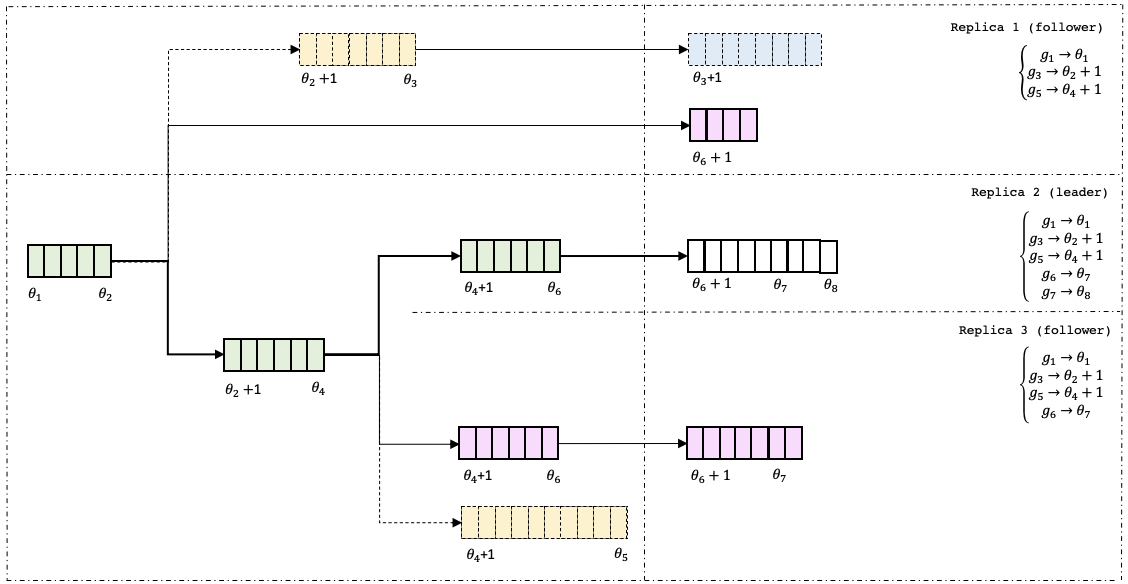
\includegraphics[scale=0.45]{lineage-tree-2.png}
	\captionof{figure}{}
	\label{fig:lineage-tree-2}
\end{figure}



\newpage
\section{Coordination for Data Tiering}

\newpage
\section{Garbage collection of orphan segments}

\newpage
\bibliographystyle{plain}
\bibliography{tiered-storage-replication}{}
\end{document}
